\documentclass{article}

% if you need to pass options to natbib, use, e.g.:
%     \PassOptionsToPackage{numbers, compress}{natbib}
% before loading neurips_2018

% ready for submission
% \usepackage{neurips_2018}

% to compile a preprint version, e.g., for submission to arXiv, add add the
% [preprint] option:
%     \usepackage[preprint]{neurips_2018}

% to compile a camera-ready version, add the [final] option, e.g.:
\usepackage[final]{main}

% to avoid loading the natbib package, add option nonatbib:
%     \usepackage[nonatbib]{neurips_2018}
\usepackage[utf8]{inputenc} % allow utf-8 input
\usepackage[T1]{fontenc}    % use 8-bit T1 fonts
\usepackage{hyperref}       % hyperlinks
\usepackage{url}            % simple URL typesetting
\usepackage{booktabs}       % professional-quality tables
\usepackage{amsmath}       % general math
\usepackage{amsfonts}       % blackboard math symbols
\usepackage{nicefrac}       % compact symbols for 1/2, etc.
\usepackage{microtype}      % microtypography
\usepackage{booktabs}
\usepackage{subfig}
\usepackage{graphicx}

\title{DL: Assignment 1}

% The \author macro works with any number of authors. There are two commands
% used to separate the names and addresses of multiple authors: \And and \AND.
%
% Using \And between authors leaves it to LaTeX to determine where to break the
% lines. Using \AND forces a line break at that point. So, if LaTeX puts 3 of 4
% authors names on the first line, and the last on the second line, try using
% \AND instead of \And before the third author name.

\author{%
  Jonathan Mitnik \\
  MSc Artificial Intelligence\\
  University of Amsterdam\\
  \texttt{jonathan@student.uva.nl} \\
}

\begin{document}
% \nipsfinalcopy is no longer used
\maketitle

\begin{abstract}
    In this report, the main focus is to go through the assignment, starting with a rough Numpy
    implementation, and then using State-of-the-art PyTorch.
\end{abstract}

\section{Derivatives}
Test123asdasdasdasdasd
asdasdasd

\section{PyTorch Implementation}
In this part of the report, results of the PyTorch experimentation are described, as well as a quick hint to the differnece between ELU and TanH.

\subsection{Experimental design: Getting the MLP to 0.52 and beyond}
In the experiment, the goal was to get the MLP to 0.52 accuracy. To do this, a number of test-cases were considered. To prevent an 
explosion of the parameter space (and learn to understand simple changes better for the scope of this project),
changes were alternated most of the time, rather than combining them together. In the following table, the results of various experiments.
To ensure an easy overview, all the cells that contain a "-" use the default parameters as provided in the original code.

Furthermore, for batchnorm, an 'X' indicates that it has been used. The batchnorm was utilized only on hidden layers,
and not on the output layer.

The best performing is the bottom row in the following table:

\begin{table}[h]
    \begin{tabular}{@{}lllllll@{}}
    \toprule
    optimizer & hidden\_layers & batchnorm & batch-size & act\_fn & max\_steps & results \\ \midrule
    -         & -              & -         & -          & -       & -          & 0.451   \\
    adam      & -              & -         & -          & -       & -          & 0.461   \\
    -         & -              & -         & 64         & -       & -          & 0.41    \\
    -         & -              & -         & 256        & -       & -          & 0.456   \\
    -         & -              & X         & -          & -       & -          & 0.412   \\
    -         & -              & -         & -          & -       & 10000      & 0.480   \\
    -         & -              & -         & -          & tanh    & -          & 0.353   \\
    -         & 64,128         & -         & -          & -       & -          & 0.426   \\
    adam      & 64,128         & -         & -          & -       & -          & 0.421   \\
    adam      & 64,128         & -         & -          & -       & 10000      & 0.462   \\
    adam      & 64, 128        & X         & -          & -       & 10000      & 0.524   \\
    adam      & 64,128,256     & X         & -          & -       & 10000      & \textbf{0.531}   \\ \bottomrule
    \end{tabular}
    \caption{Runs with various permutations}
\end{table}

\begin{figure}%
    \centering
    \subfloat[\centering Training loss for default settings]{{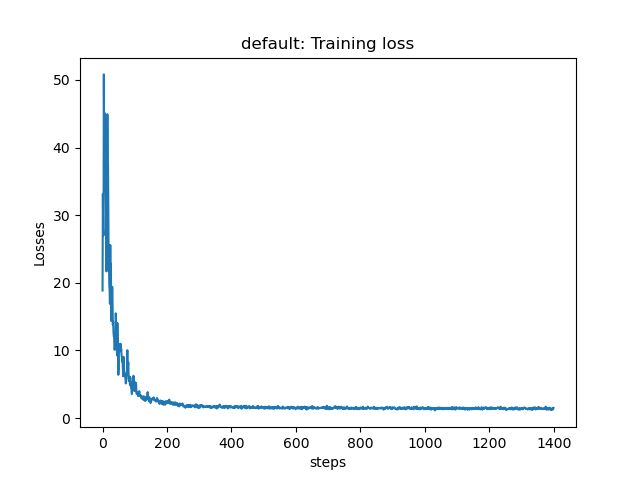
\includegraphics[width=6.5cm]{images/pytorch-mlp-default.train_loss.png} }}%
    \qquad
    \subfloat[\centering Test accuracy for default settings]{{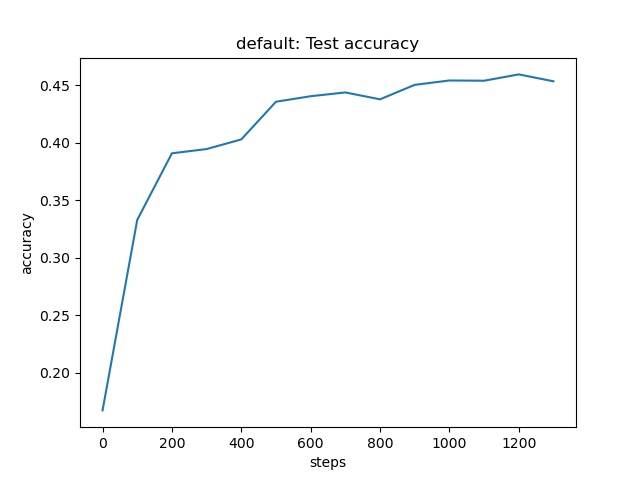
\includegraphics[width=6.5cm]{images/pytorch-mlp-default_test_accs.png} }}%
    \caption{Default performance, test and train}%
    \label{fig:defaults}%
\end{figure}

\begin{figure}%
    \centering
    \subfloat[\centering Training loss for best settings]{{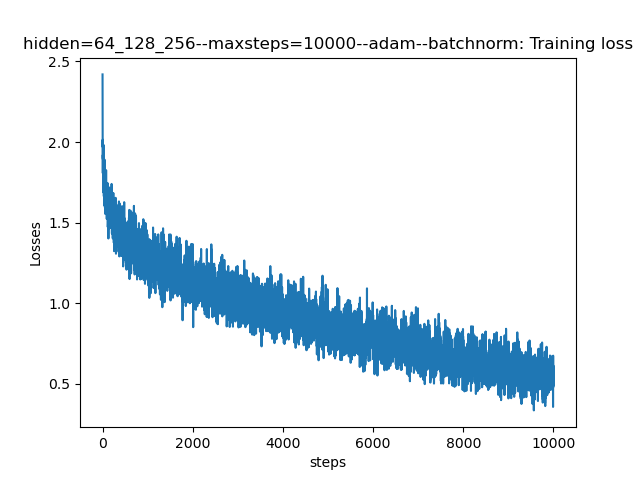
\includegraphics[width=6.5cm]{images/pytorch-mlp-hidden=64_128_256--maxsteps=10000--adam--batchnorm.train_loss.png} }}%
    \qquad
    \subfloat[\centering Test accuracy for best settings]{{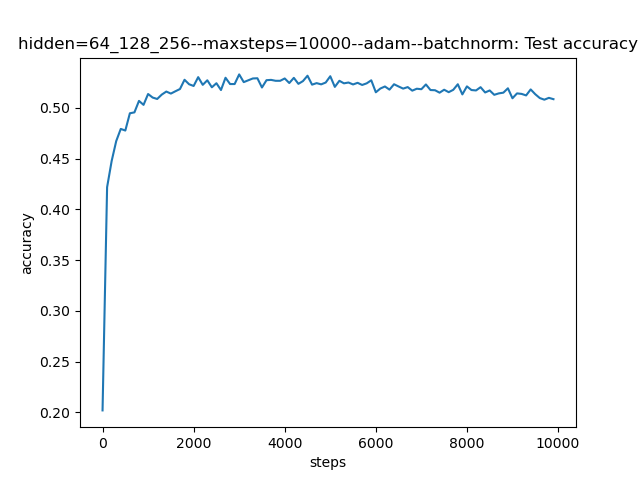
\includegraphics[width=6.5cm]{images/pytorch-mlp-hidden=64_128_256--maxsteps=10000--adam--batchnorm.test_accs.png} }}%
    \caption{Best performance, test and train}%
    \label{fig:defaults}%
\end{figure}

In the end, the best performance turned out to be the inclusion of batch-norm with more steps and more layers.
Important to note, was that especially when adding batch-norm, the ability to generalize with more layers started improving
tremendously.

\subsection{ELU vs TanH}
Some of the main benefits of using TanH, is that it provides a very clear bound for the activation values. 
ELU has no upper boundary, meaning that values could theroretically become huge, and rely on regularization
techniques. 

Drawbacks of Tanh relate to both slightly more expensive computation of the gradient of Tanh (more complex than
the very simple form of the ELU), and the dense layer weights it allows. With ELU, many insignificant weights
go to practically 0, whereas with Tanh, the weights are scaled somewhere between -1 and 1. Furthermore, 
networks with Tanh activation functions have converged a lot slower in this example for instance. 

Tanh could be used for outputting your values to a particular characteristic (e.g [-1, 1]). If the output
of your model requires this, Tanh can be used. ELU should never be used as output activation for your network.

\section{Layer normalization}
\subsection*{3.2a: Manual implementation of backward pass}
I will start by writing down, in essence, all known shapes.

\begin{enumerate}
    \item $\emph{\textbf{X}} \in \mathbb{R}^{S * M}$
    \item $\emph{\textbf{Y}} \in \mathbb{R}^{S * M}$ (same shape as X)
    \item $L \in \mathbb{R}^{1}$
    \item $\gamma \in \mathbb{R}^{M}$
    \item $\beta \in \mathbb{R}^{M}$
    \item $\frac{\delta L}{\delta \gamma} \in \mathbb{R}^{M}$
    \item $\frac{\delta L}{\delta \beta} \in \mathbb{R}^{M}$
    \item $\frac{\delta L}{\delta \emph{\textbf{Y}}} \in \mathbb{R}^{S * M}$
    \item $\frac{\delta L}{\delta \emph{\textbf{X}}} \in \mathbb{R}^{S * M}$
\end{enumerate}

To start, the first derivative we calculate is that of $\frac{\delta L}{\delta \gamma}$.

% DL_dgamma
% TODO: How do we get to the full form again?
{\Large $\frac{\delta L}{\delta \gamma}$ }:
\boxed{\begin{aligned}
    \frac{\delta L}{\delta \gamma}
    &=> [\frac{\delta L}{\delta \gamma}]_i
    = \frac{\delta L}{\delta \gamma}_i
    = \sum_{sj} \frac{\delta L}{\delta Y_{sj}} * \frac{\delta Y_{sj}}{\delta \gamma_i} \\
    % Now we start
    &= \sum_{sj} \frac{\delta L}{\delta Y_{sj}} 
        * \frac{\delta \gamma_j \hat{X}_{sj}}{\delta \gamma_i} \\
    &= \sum_{sj} \frac{\delta L}{\delta Y_{sj}} 
        * \delta_{ji} \hat{X}_{sj} \\
    &= \sum_{s} \frac{\delta L}{\delta Y_{si}} 
        * \hat{X}_{si} \\
    &= \sum_{s} \textbf{1}_s*  \frac{\delta L}{\delta Y_{si}} 
        * \hat{X}_{si} \\
    &=> \textbf{1}^T * [\frac{\delta L}{\delta Y} 
        \circ \hat{X}] && \text{where $$\textbf{1}$$ is a 1xS vector} \\
\end{aligned}}

\vspace{1cm}
In a similar way we can calculate the derivative with respect to $\beta$.

% DL_dbeta
% TODO: How do we get to the full form again?
{\Large $\frac{\delta L}{\delta \beta}$ }:
\boxed{\begin{aligned}
    \frac{\delta L}{\delta \beta}
    &=> [\frac{\delta L}{\delta \beta}]_i
    = \frac{\delta L}{\delta \beta}_i
    = \sum_{sj} \frac{\delta L}{\delta Y_{sj}} * \frac{\delta Y_{sj}}{\delta \beta_i} \\
    % Now we start
    &= \sum_{sj} \frac{\delta L}{\delta Y_{sj}} 
        * \frac{\delta \gamma_j \hat{X}_{sj} + \beta_J}{\delta \beta_i} \\
    &= \sum_{sj} \frac{\delta L}{\delta Y_{sj}} 
        * \delta_{ji} \\
    &= \sum_{s} \frac{\delta L}{\delta Y_{si}} \\
    &= \textbf{1}^T * \frac{\delta L}{\delta Y} && \text{where $$\textbf{1}$$ is a 1xS vector} \\
\end{aligned}}

\vspace{1cm}
Now on to calculating the derivative with respect to $X$. It would be good to first define the starting chain:

\begin{align}
    \frac{\delta L}{\delta \textbf{\emph{X}}}
    &=> \frac{\delta L}{\delta X_{ri}}
    = \sum_{sj} \frac{\delta L}{\delta Y_{sj}} * \frac{\delta Y_{sj}}{\delta X_{ri}}
\end{align}

When focusing on $\frac{\delta Y_{sj}}{\delta X_{ri}}$, there are a number of aspects that come to play. 
To start, we can break it down into a chain, where we explicitly focus on the "contribution"
that $\mu$ and $\sigma$ have on X.

\begin{align}
    \frac{\delta Y_{sj}}{\delta X_{ri}} &= 
        % Directly X first
        \frac{\delta Y_{sj}}{\delta \hat{X}_{sj}} * \frac{\delta \hat{X}_{sj}}{\delta X_{ri}}
            + \frac{\delta Y_{sj}}{\delta \mu_j} * \frac{\delta \mu_j}{\delta X_{ri}}
            + \frac{\delta Y_{sj}}{\delta \sigma^2_j} * \frac{\delta \sigma^2_j}{\delta X_{ri}}
\end{align}

This contains quite a number of steps

\section{Conv nets}
In this section, a simple and light-weight version of the Resnet version has been implemented, trained and evaluated.
\begin{figure}%
    \centering
    \subfloat[\centering Training loss for Convnet]{{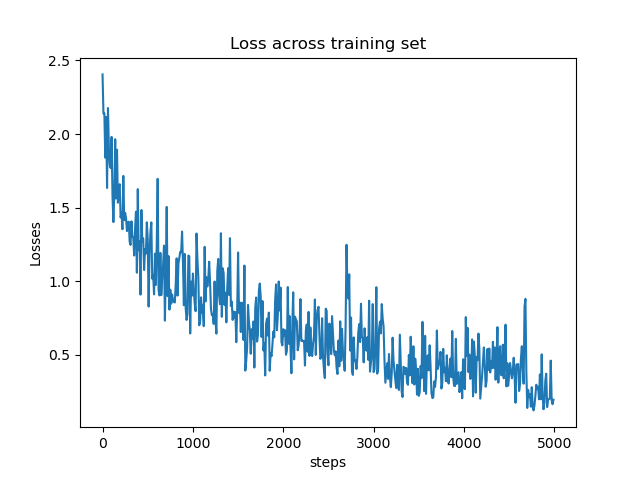
\includegraphics[width=6.5cm]{images/convnet-train_loss.png} }}%
    \qquad
    \subfloat[\centering Test accuracy for Convnet]{{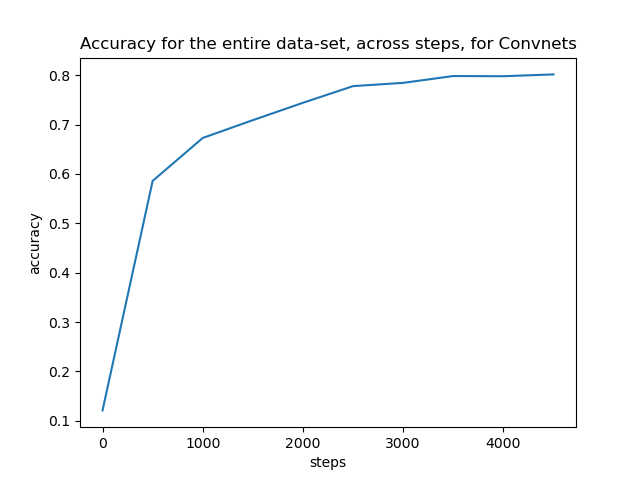
\includegraphics[width=6.5cm]{images/convnet-test_accs.png} }}%
    \caption{Default performance, test and train, for Convnet}%
    \label{fig:defaults}%
\end{figure}

By the end of the default number of steps, the model was not necessarily showing any sign of "stopping". 
What is interesting to note, is that the model seems to reach a point where the accuracy's linear increase (around 800 steps as seen in testing scores)
slopes down a bit. While it does not reach convergence yet, it seems that from this point the model slows down
its learning considerably; this is likely a decrease in learning rate as set by Adam's optimizer.

It is surprising nonetheless how fast this model learns on "limited" data. The gradients are not vanished,
due to the resnet blocks, which means that even the deeper layers get enough of a signal to keep training.

The loss curve here (admittedly, I should have used averaged scores over steps, but time constraints and LISA server errors proved an extra challenge to run on time again)
indicates "hops": around step 700, 1500, 3000, and 4700, the loss make significant "average" drops.

\end{document}